\documentclass[11pt]{article}
\usepackage[margin=1in]{geometry}
\usepackage{enumitem}
\usepackage{hyperref}
\usepackage{graphicx}
\usepackage{array}
\usepackage{multicol}
\usepackage{longtable}
\usepackage{titlesec}
\usepackage{float}

\begin{document}

%==================================================
\begin{center}
    \large \textbf{Sri Sivasubramaniya Nadar College of Engineering, Chennai} \\
    (An autonomous Institution affiliated to Anna University) \\
    \vspace{0.3cm}
\end{center}

\begin{table}[!h]
\renewcommand{\arraystretch}{1.5}
\resizebox{\textwidth}{!}{%
\begin{tabular}{|l|cll|}
\hline
Degree \& Branch & \multicolumn{1}{c|}{B.E. Computer Science \& Engineering} & Semester & VI \\ \hline
Subject Code \& Name & \multicolumn{3}{c|}{UCS2612 -- Machine Learning Algorithms Laboratory} \\ \hline
Academic Year & \multicolumn{1}{c|}{2025--2026 (Even)} & Batch & 2023--2027 \\ \hline
Name & Prawin Kumar S & Register No. & 3122235001100 \\ \hline
Due Date & \multicolumn{3}{c|}{27 January 2026} \\ \hline
\end{tabular}
}
\end{table}

\begin{center}
\textbf{Experiment 2: Binary Classification using Na\"ive Bayes and K-Nearest Neighbors}
\end{center}

%==================================================
\section*{1. Aim and Objective}
To implement and comprehensively evaluate Na\"ive Bayes and K-Nearest Neighbors (KNN) classifiers for binary classification tasks. The experiment involves analyzing multiple performance metrics across different algorithm variants, visualizing model behavior through various graphical representations, and conducting in-depth analysis of overfitting and underfitting phenomena. Additionally, the study examines bias-variance tradeoffs inherent in both parametric and non-parametric classification approaches, providing insights into their practical applicability and computational efficiency.

%==================================================
\section*{2. Dataset Description}
The experiment utilizes the Spambase dataset, a benchmark binary classification dataset from the UCI Machine Learning Repository, widely recognized for email spam detection research.

Dataset reference:
\begin{itemize}
    \item Kaggle: \href{https://www.kaggle.com/datasets/somesh24/spambase}{Spambase Dataset}
    \item UCI Machine Learning Repository
\end{itemize}

The Spambase dataset comprises 4,601 email instances, each characterized by 57 continuous real-valued attributes representing the frequency of specific words and characters commonly associated with spam messages. These features include word frequencies for terms such as 'free', 'money', 'business', and character frequencies for special symbols like '!', '\$', and '\#'. The target variable is binary, with class label 1 indicating spam emails and 0 representing legitimate (non-spam) emails. The dataset exhibits a moderate class imbalance, with approximately 39.4\% spam instances and 60.6\% non-spam instances, reflecting realistic email distribution patterns. This imbalance necessitates careful evaluation using metrics beyond simple accuracy to ensure robust model performance assessment.

%==================================================
\section*{3. Preprocessing Steps}
The preprocessing pipeline was systematically designed to prepare the data for optimal classifier performance:

\begin{enumerate}
    \item \textbf{Data Integrity Verification}: A comprehensive missing value analysis was conducted across all 57 features and 4,601 instances. The dataset was found to be complete with no missing values, eliminating the need for imputation strategies.
    
    \item \textbf{Stratified Data Splitting}: The dataset was partitioned into training (70\%, 3,220 instances) and testing (30\%, 1,381 instances) subsets using stratified random sampling. This approach ensures that the original class distribution is preserved in both sets, maintaining approximately 39.4\% spam and 60.6\% non-spam ratios, which is critical for unbiased model evaluation.
    
    \item \textbf{Feature Scaling and Normalization}:
    \begin{itemize}
        \item \textbf{Min-Max Normalization}: Applied specifically for Multinomial Na\"ive Bayes implementation, transforming all feature values to the range [0, 1]. This transformation is essential because Multinomial Na\"ive Bayes requires non-negative feature values and interprets them as frequency counts or proportions.
        
        \item \textbf{Standardization (Z-score Normalization)}: Employed for Gaussian Na\"ive Bayes and KNN classifiers, transforming features to have zero mean and unit variance. This preprocessing step is particularly crucial for distance-based algorithms like KNN, where features with larger scales can disproportionately influence distance calculations and classification decisions.
    \end{itemize}
    
    \item \textbf{Feature Distribution Analysis}: Examined the statistical properties of features including skewness, kurtosis, and outlier presence to inform algorithm selection and parameter tuning decisions.
\end{enumerate}

%==================================================
\section*{4. Implementation Details}
The experimental framework encompassed multiple classifier variants with systematic hyperparameter optimization strategies:

\subsection*{4.1 Na\"ive Bayes Variants}
Three distinct variants of Na\"ive Bayes were implemented using Scikit-learn library:
\begin{itemize}
    \item \textbf{Gaussian Na\"ive Bayes}: Assumes features follow normal distributions within each class. This variant is suitable when features exhibit continuous, bell-shaped distributions.
    
    \item \textbf{Multinomial Na\"ive Bayes}: Models features as multinomial distributions, commonly used for discrete count data. Particularly effective for text classification and frequency-based features.
    
    \item \textbf{Bernoulli Na\"ive Bayes}: Treats features as binary (presence/absence) indicators. Useful when features represent binary occurrences rather than continuous frequencies.
\end{itemize}

\subsection*{4.2 K-Nearest Neighbors Optimization}
For the KNN classifier, extensive hyperparameter tuning was conducted to identify optimal configuration:

\textbf{Hyperparameter Search Strategies:}
\begin{itemize}
    \item \textbf{Grid Search with Cross-Validation}: Performed exhaustive search over the parameter space, evaluating all combinations of $k$ values in range [1, 30] with two weighting schemes ('uniform' and 'distance'). Five-fold cross-validation was employed to ensure robust parameter selection and prevent overfitting to the training set.
    
    \item \textbf{Randomized Search}: Implemented as an efficient alternative to grid search, randomly sampling parameter combinations from specified distributions. This approach provides computational efficiency while maintaining high probability of finding near-optimal parameters.
\end{itemize}

\textbf{Distance Metrics and Data Structures:}
\begin{itemize}
    \item Evaluated Euclidean and Manhattan distance metrics for neighbor identification
    \item Compared KDTree and BallTree spatial data structures for efficient neighbor search
    \item KDTree performs optimally for low to medium dimensional data (typically $d < 20$)
    \item BallTree excels in higher dimensions and with non-Euclidean metrics
\end{itemize}

%==================================================
\section*{5. Visualizations}

\subsection*{5.1 Exploratory Data Analysis}

\begin{figure}[H]
\centering
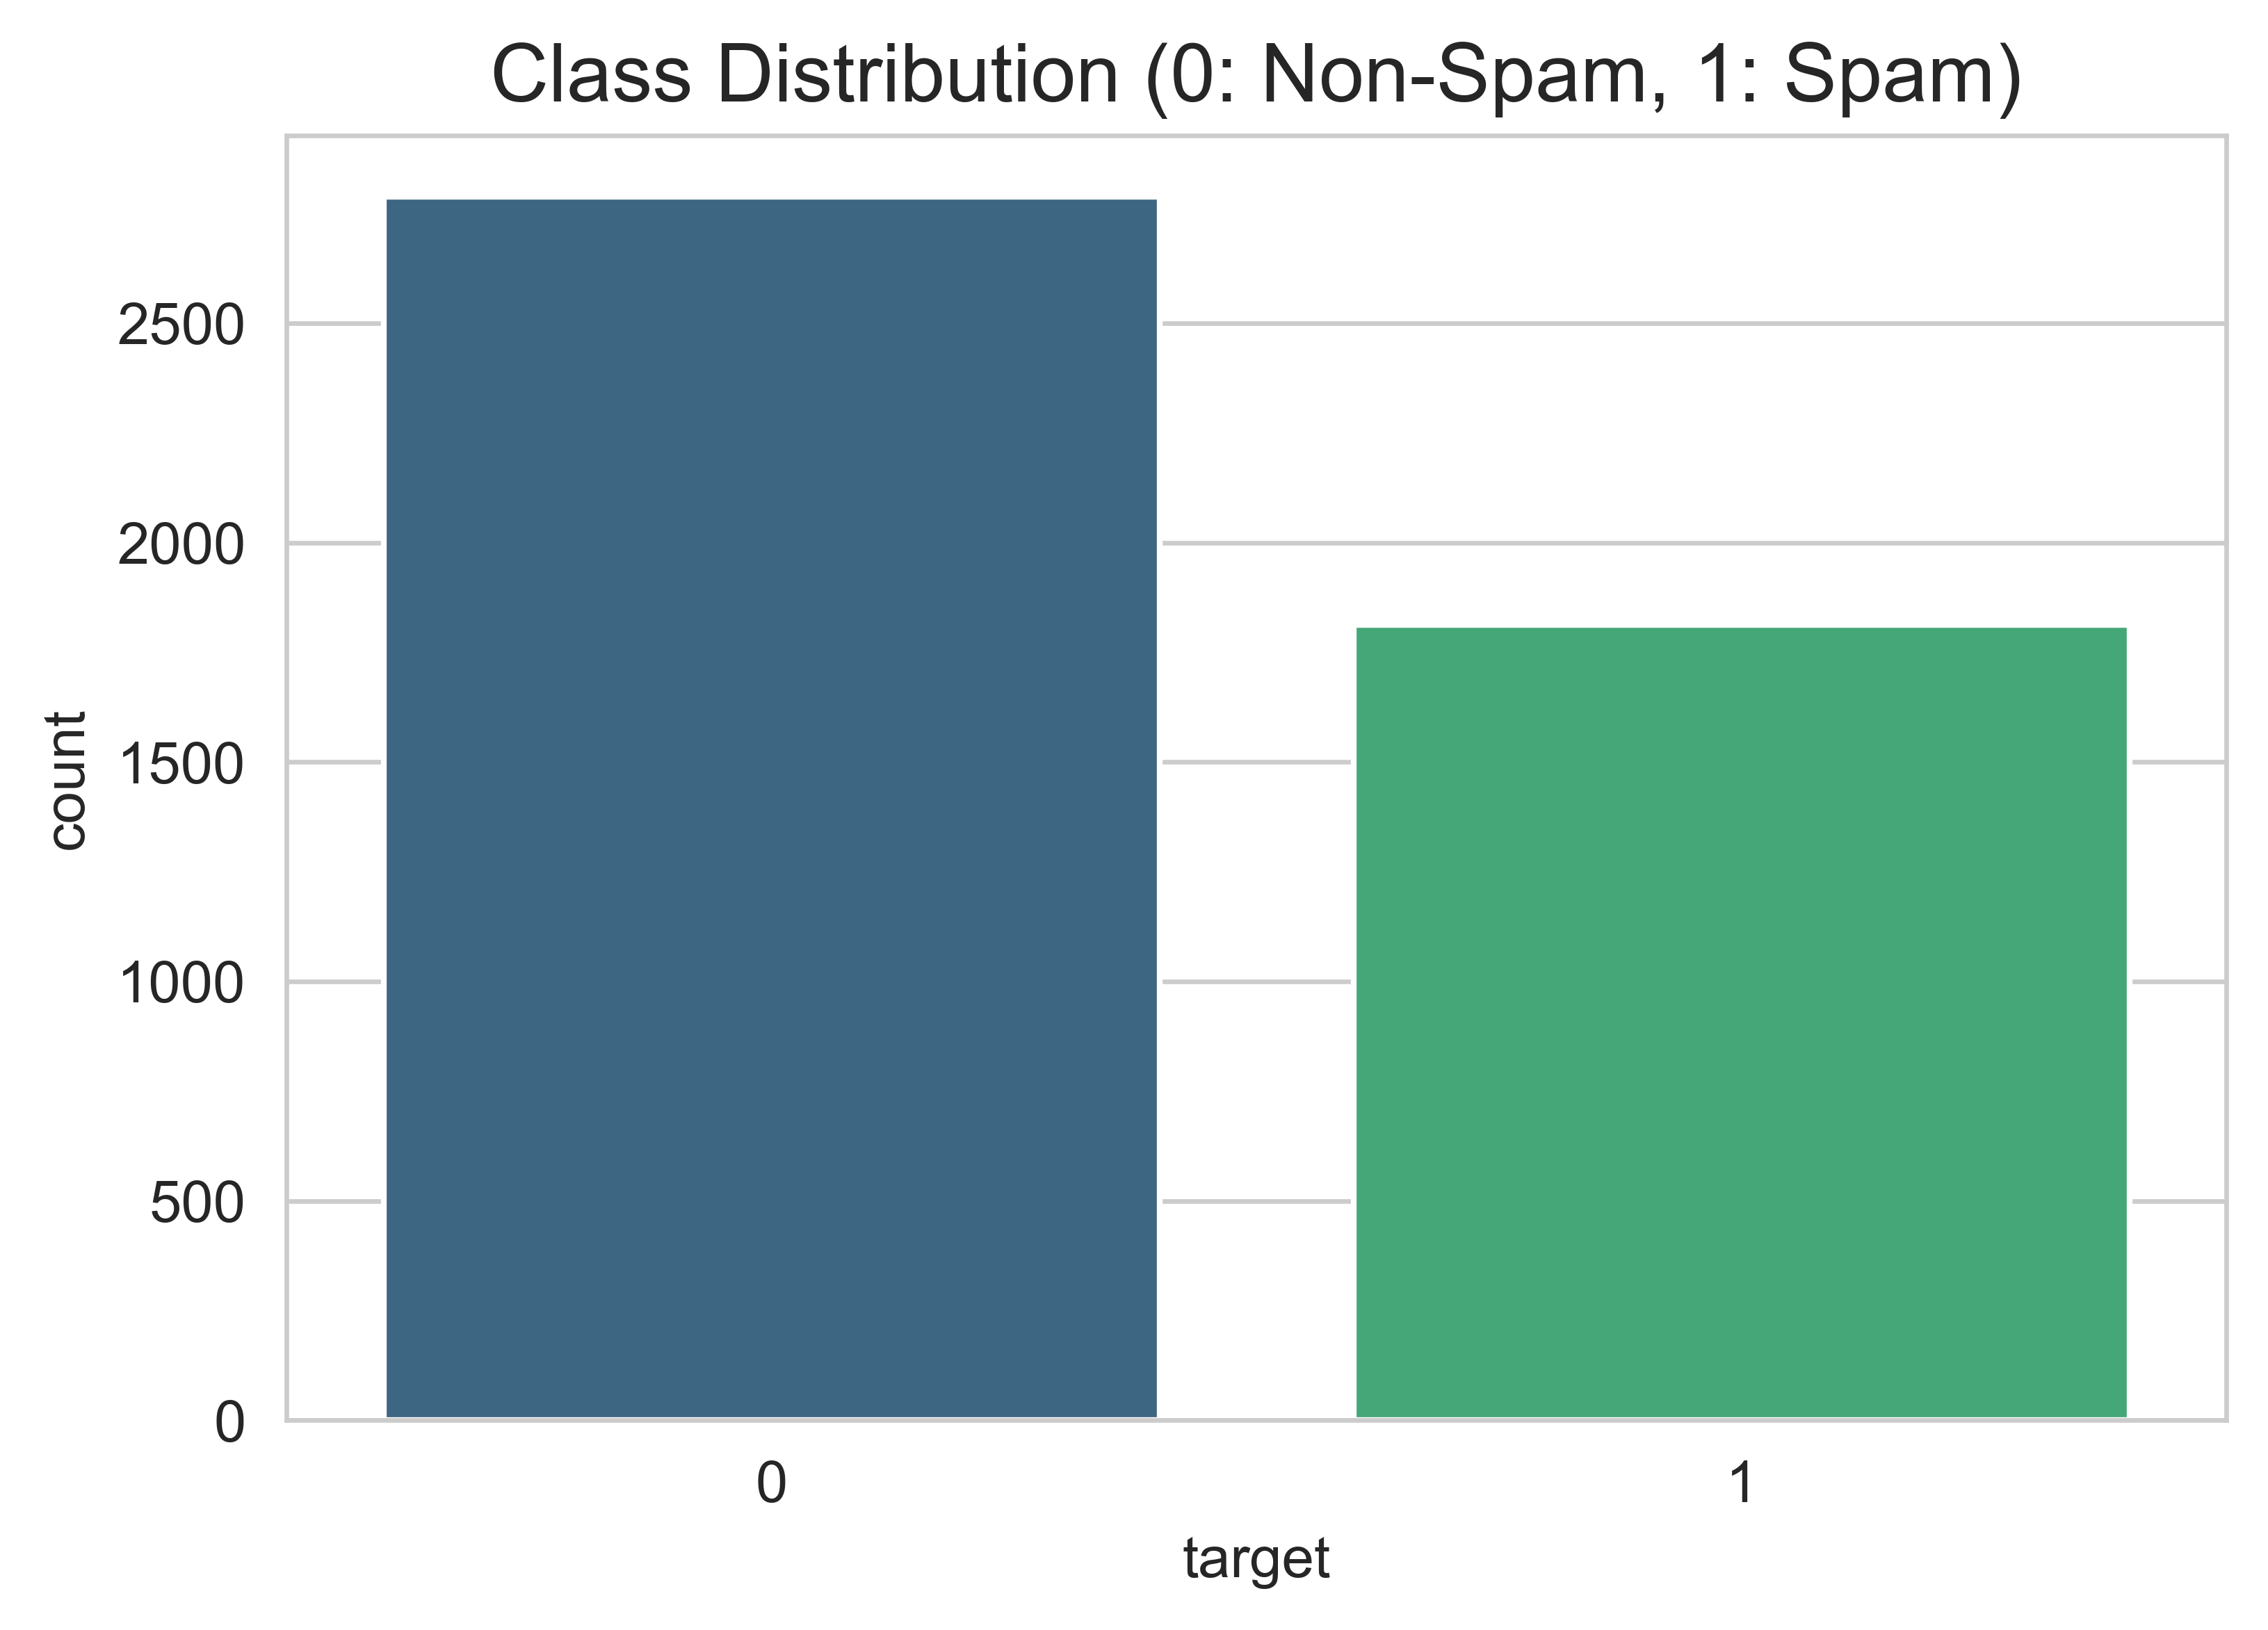
\includegraphics[width=0.7\textwidth]{png/class_distribution.png}
\caption{Class Distribution Showing Dataset Imbalance}
\end{figure}

\begin{figure}[H]
\centering
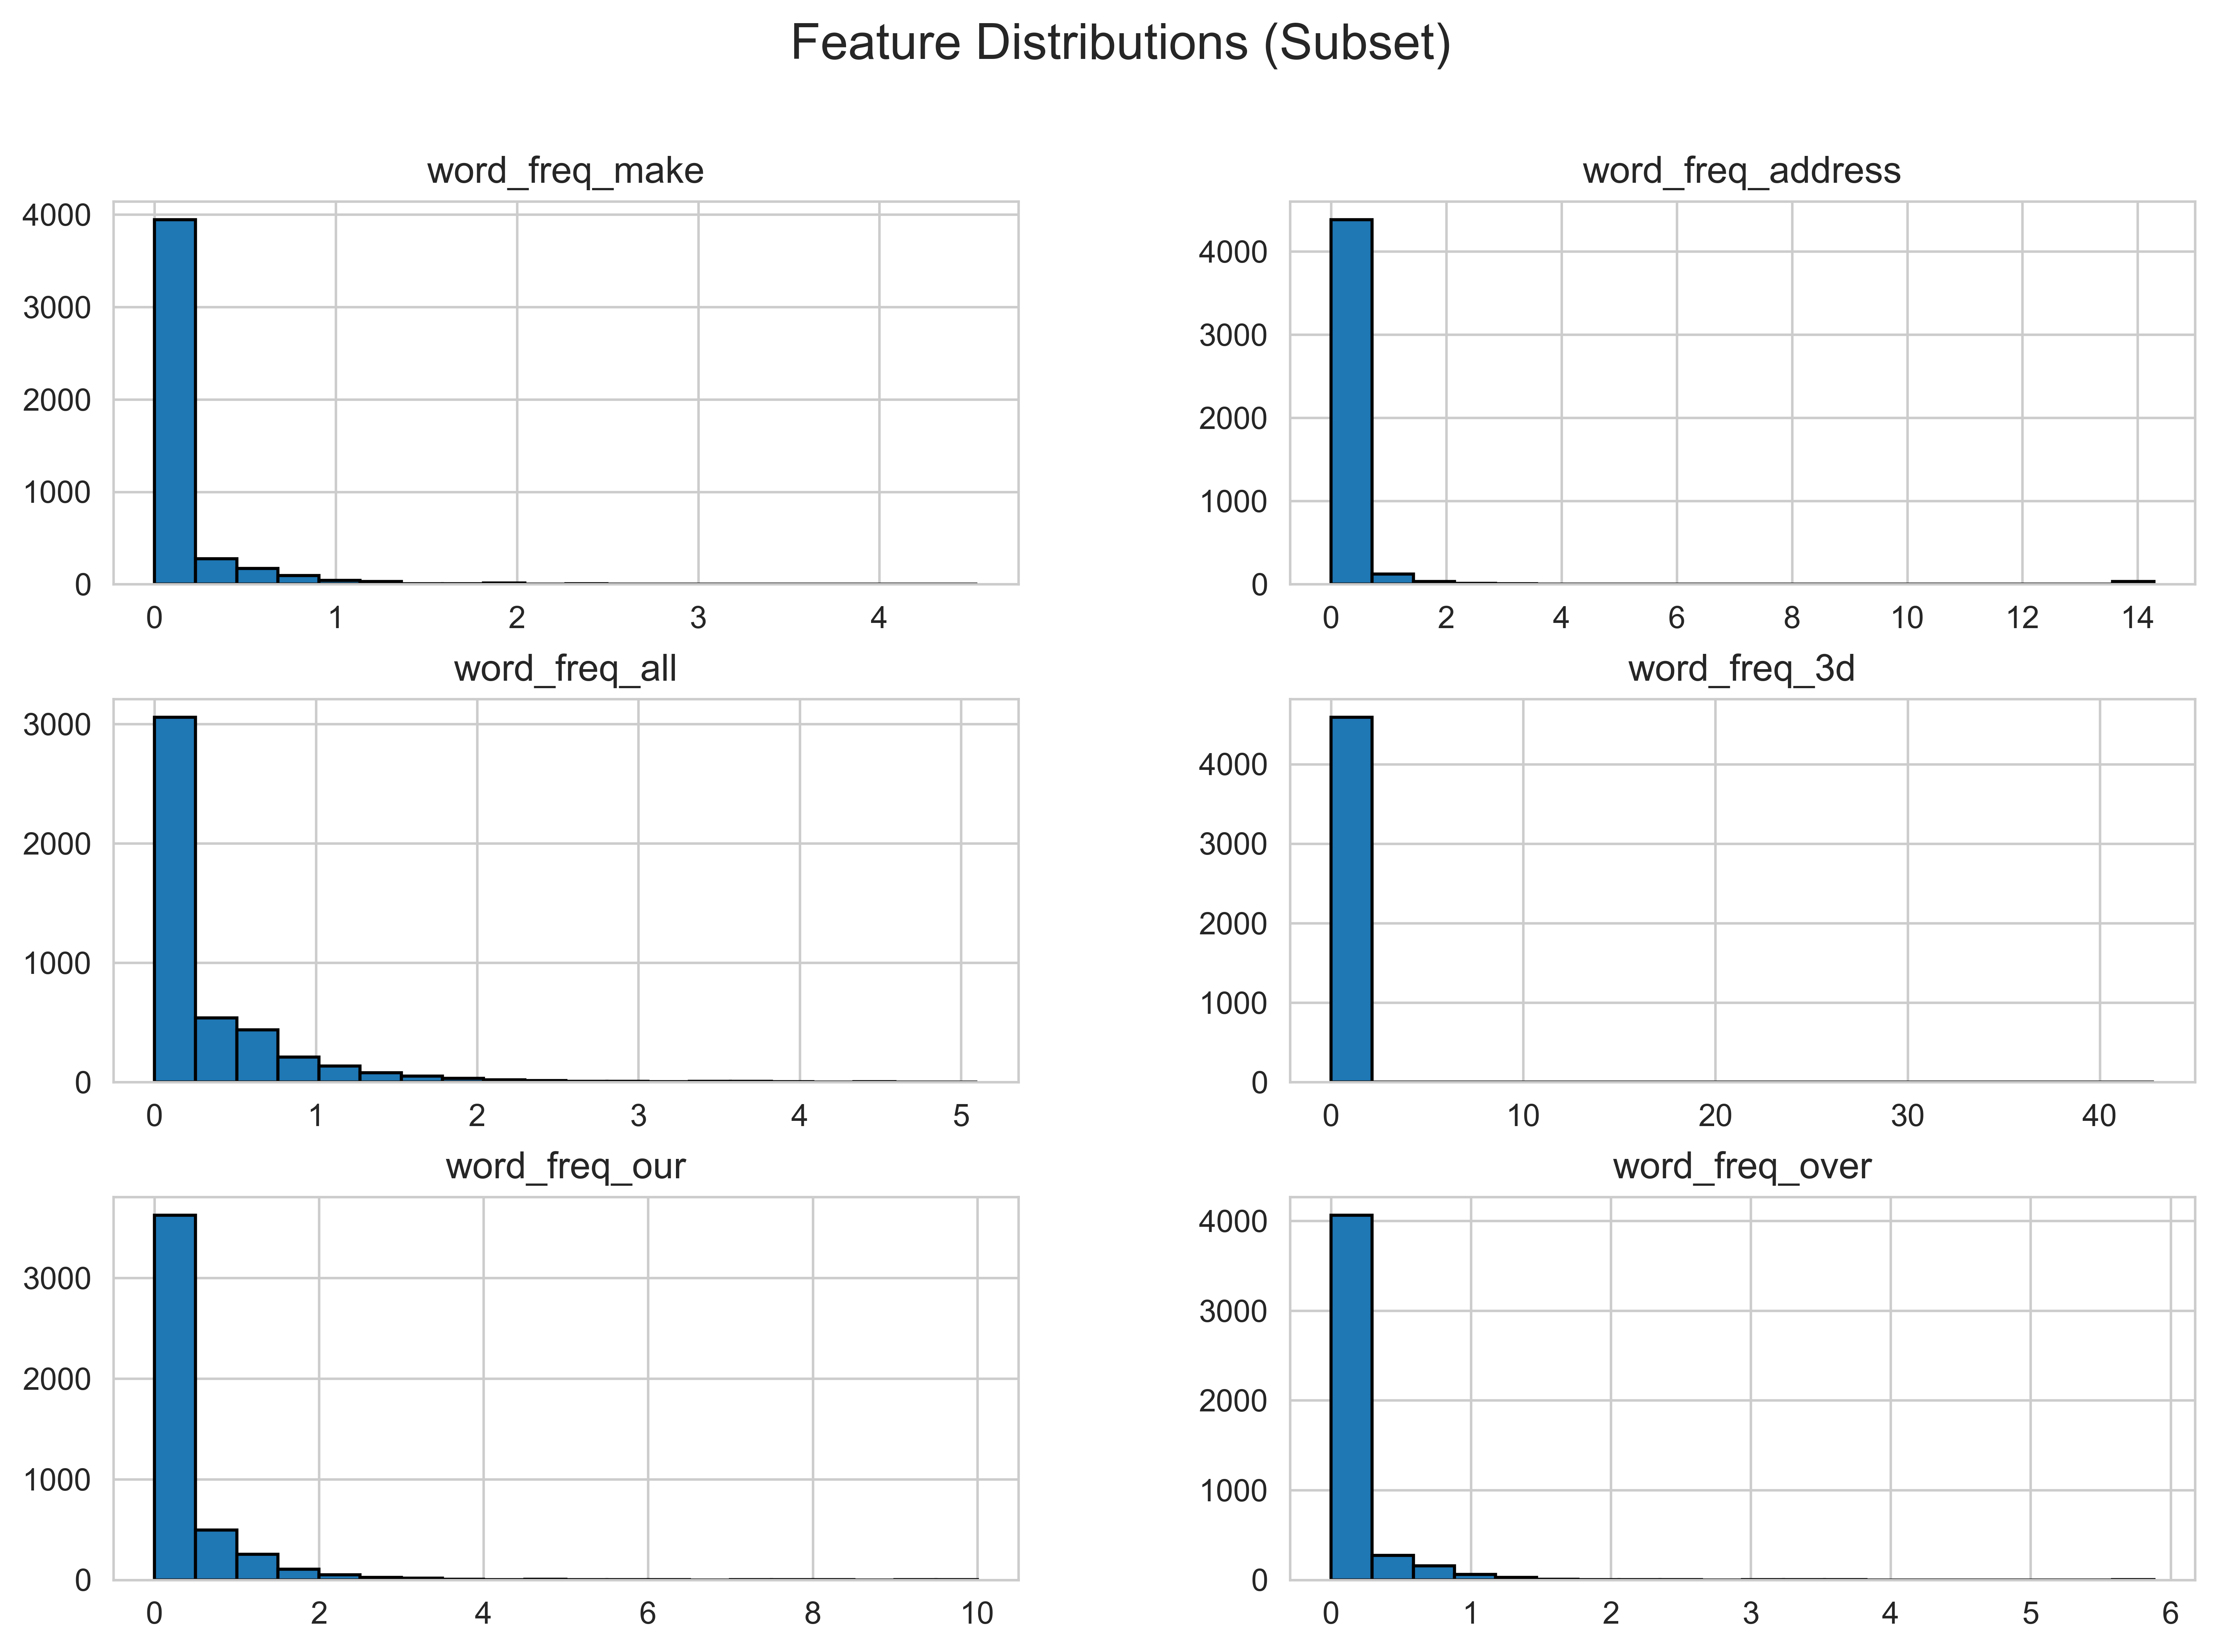
\includegraphics[width=0.9\textwidth]{png/feature_distribution.png}
\caption{Statistical Distribution of Selected Features}
\end{figure}

\subsection*{5.2 Model Evaluation and Performance Visualization}

\begin{figure}[H]
\centering
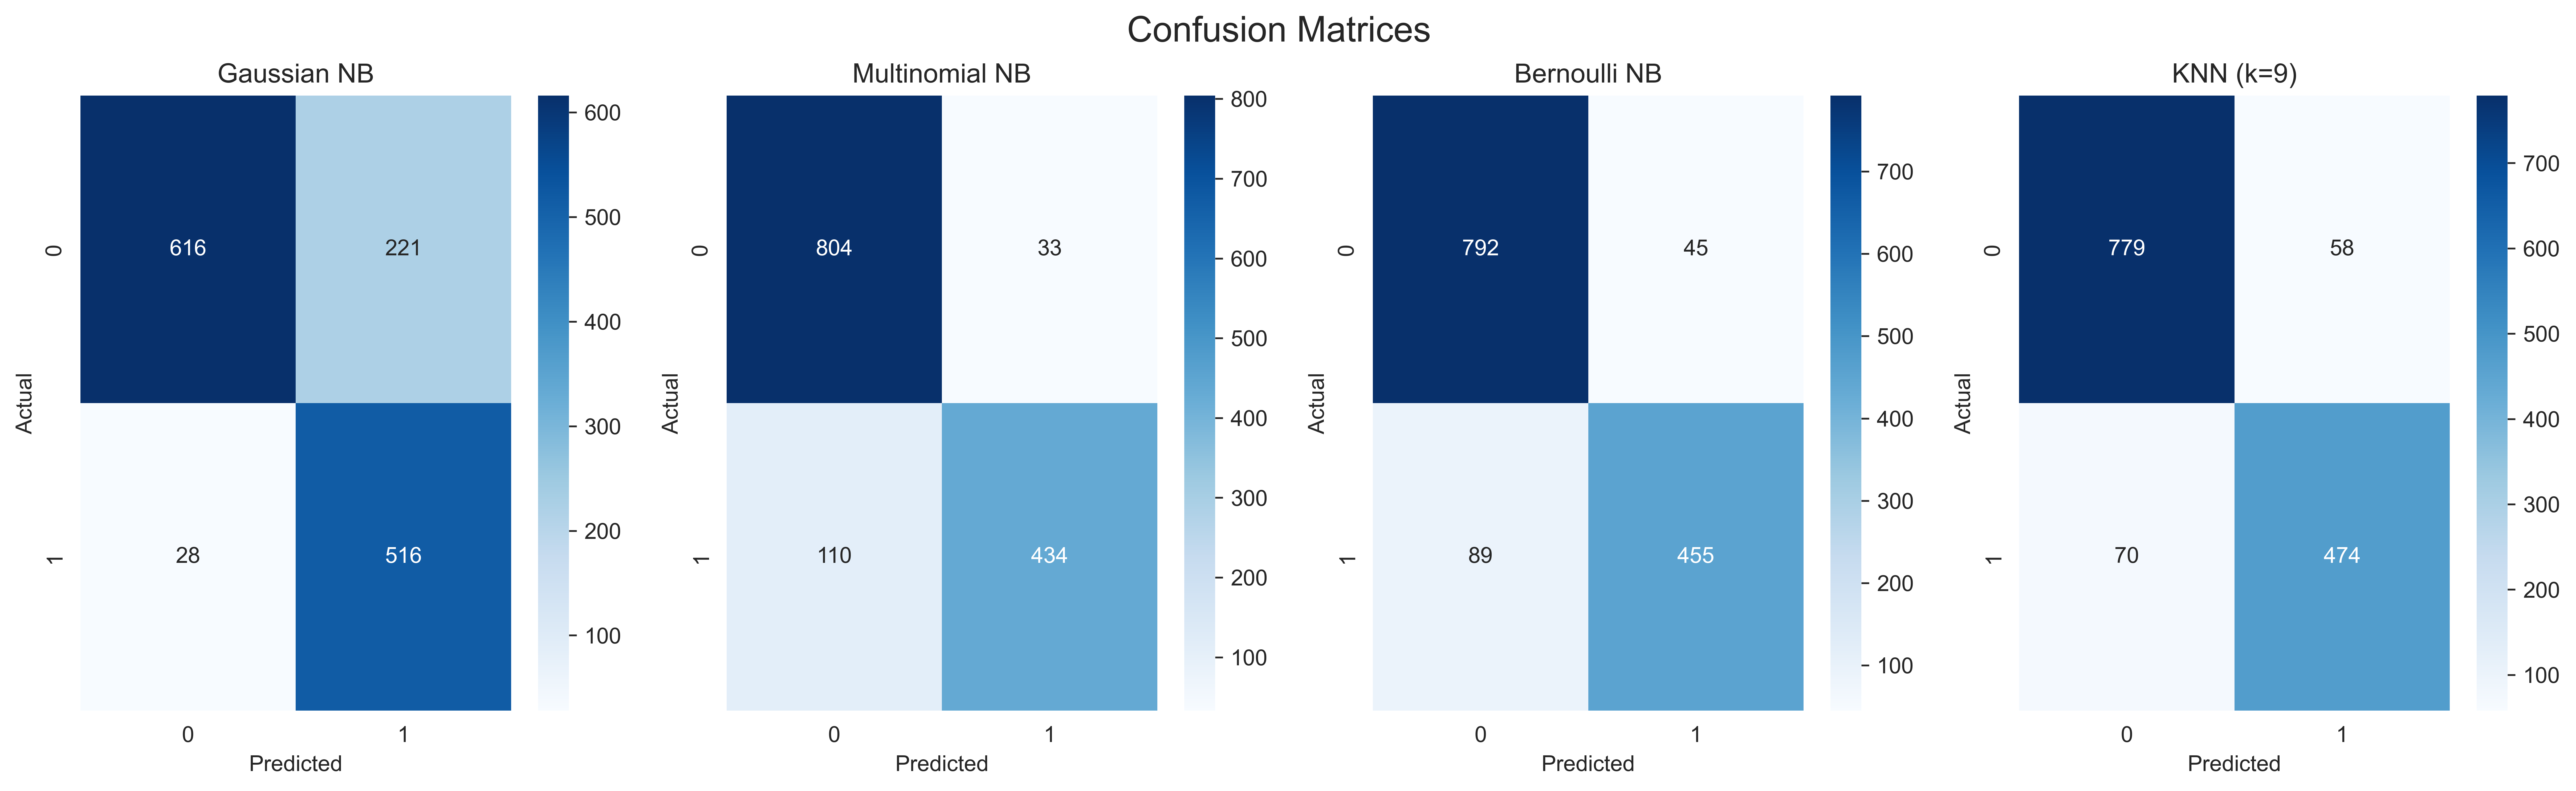
\includegraphics[width=0.9\textwidth]{png/confusion_matrices.png}
\caption{Confusion Matrices for All Classifiers}
\end{figure}

\begin{figure}[H]
\centering
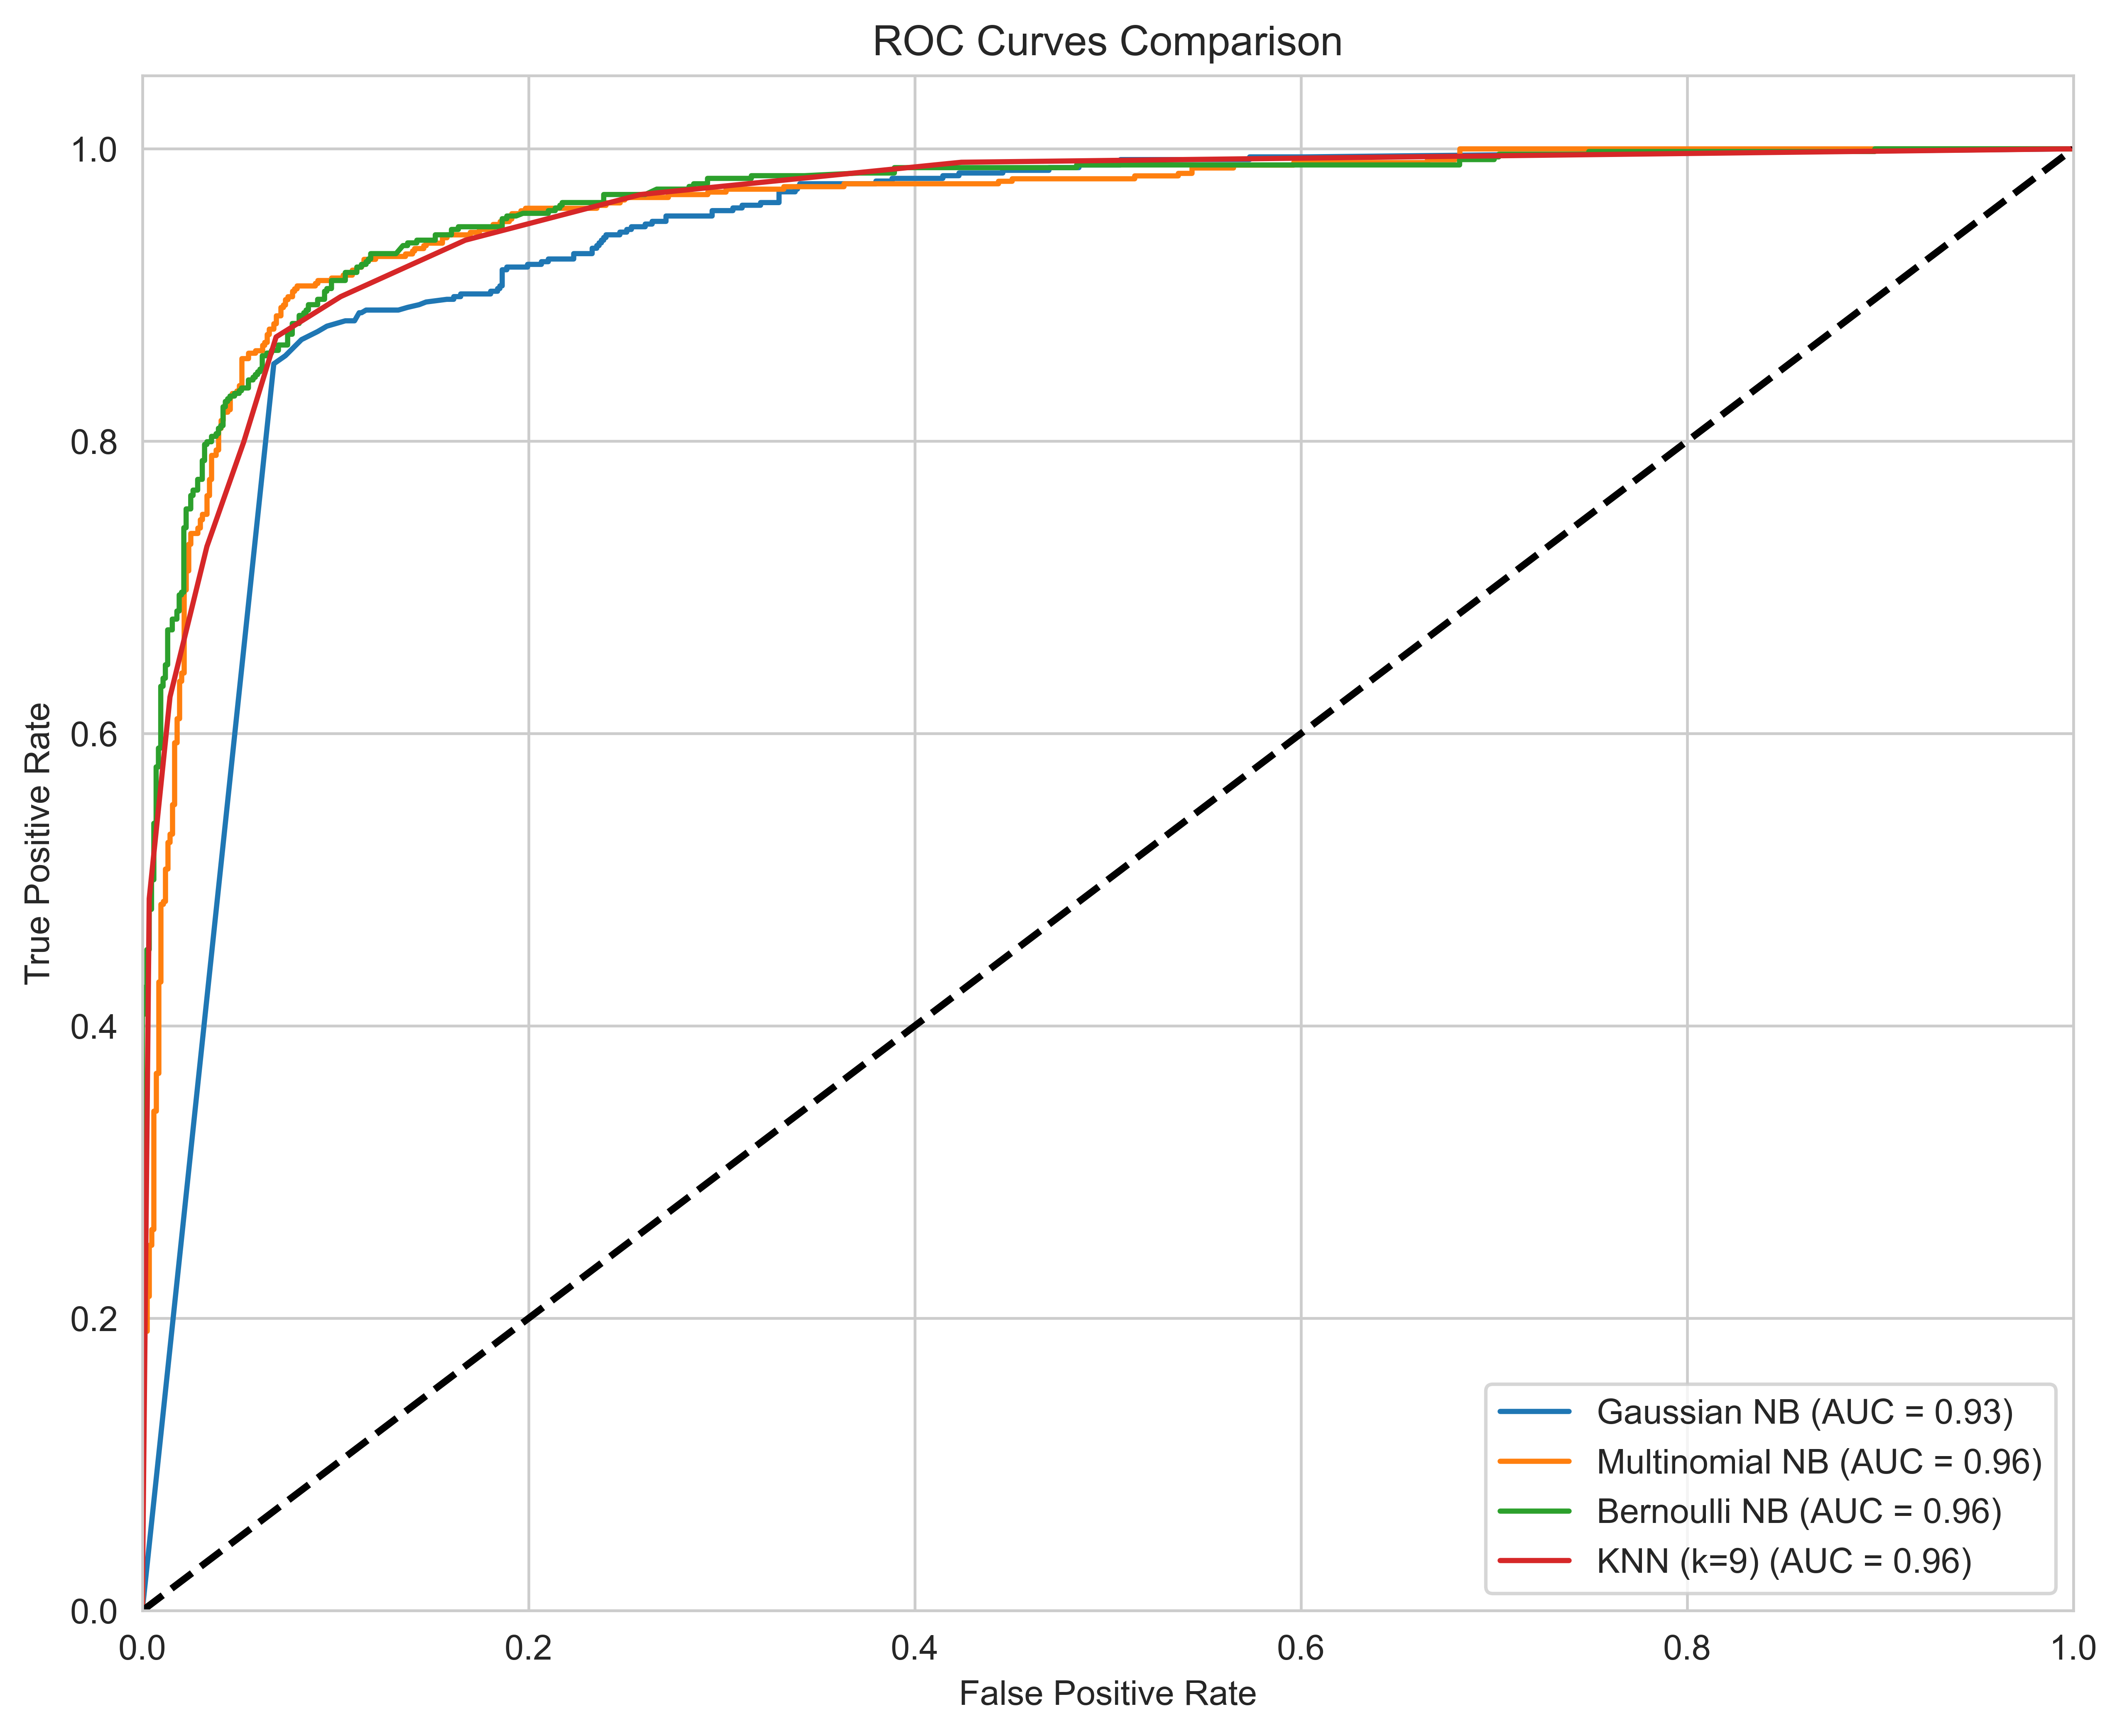
\includegraphics[width=0.8\textwidth]{png/roc_curves.png}
\caption{ROC Curves and AUC Comparison Across Classifiers}
\end{figure}

\begin{figure}[H]
\centering
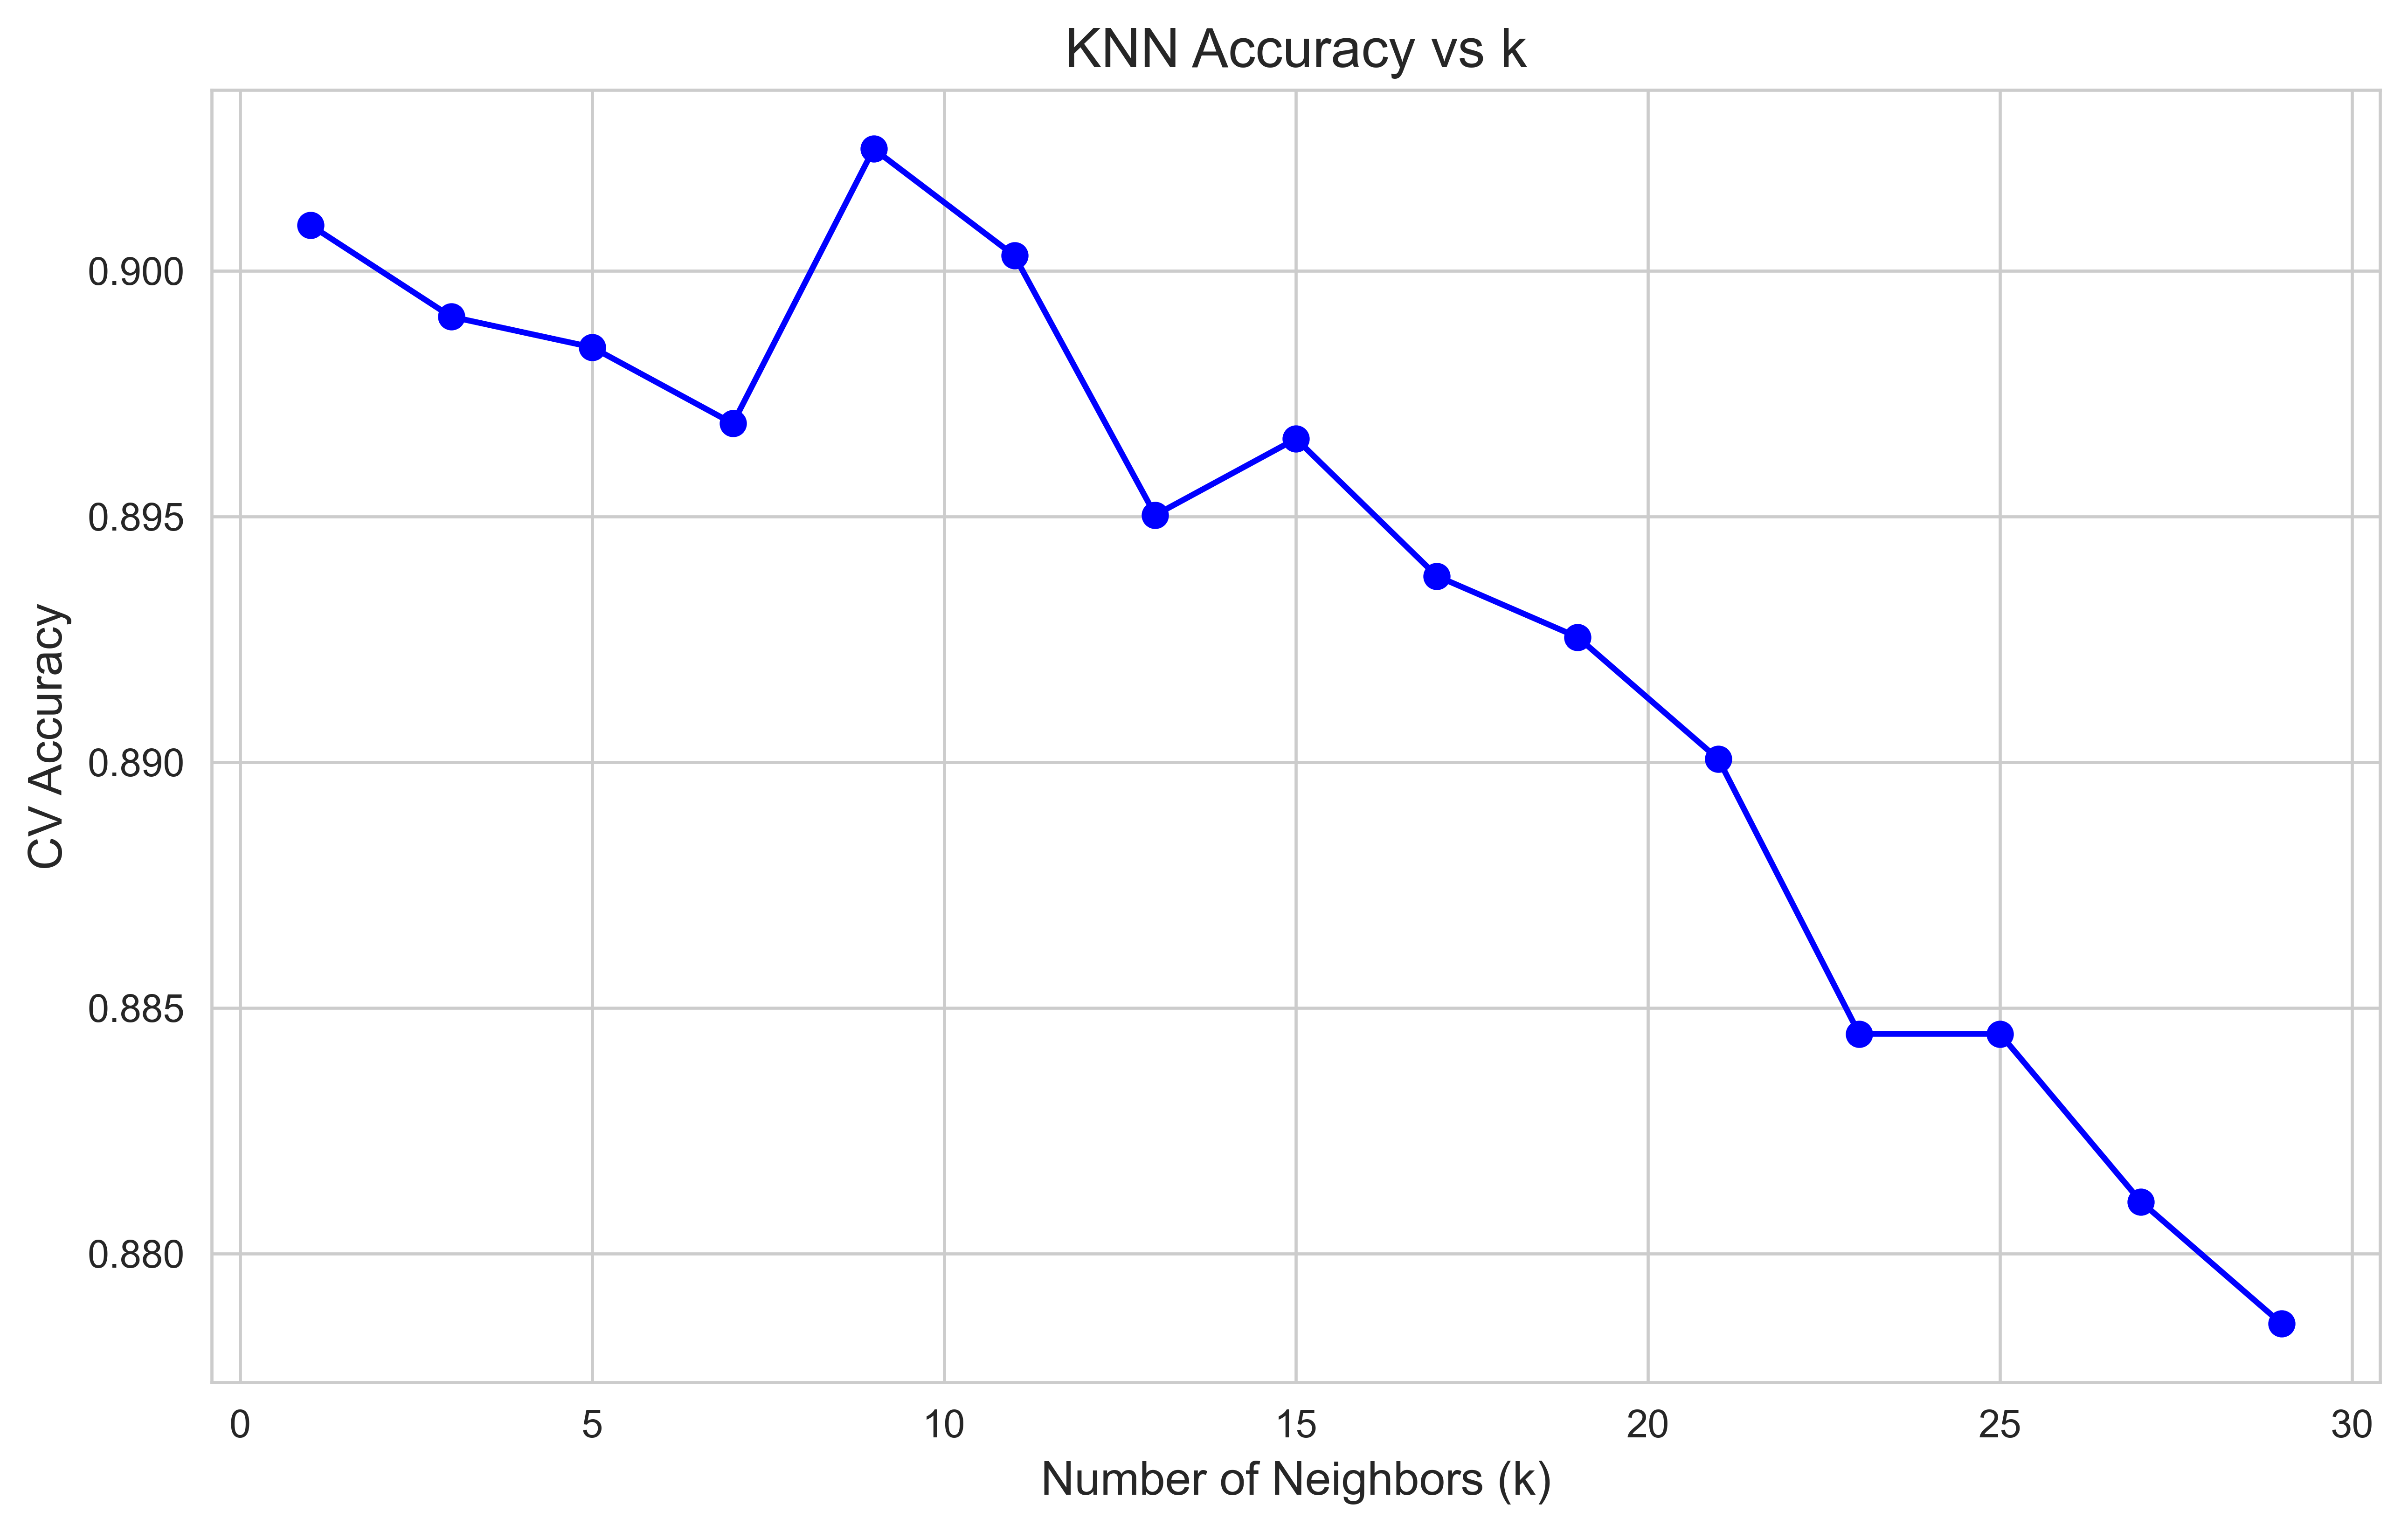
\includegraphics[width=0.8\textwidth]{png/knn_accuracy_vs_k.png}
\caption{KNN Classification Accuracy as a Function of k}
\end{figure}

\subsection*{5.3 Bias-Variance Analysis and Learning Curves}

\begin{figure}[H]
\centering
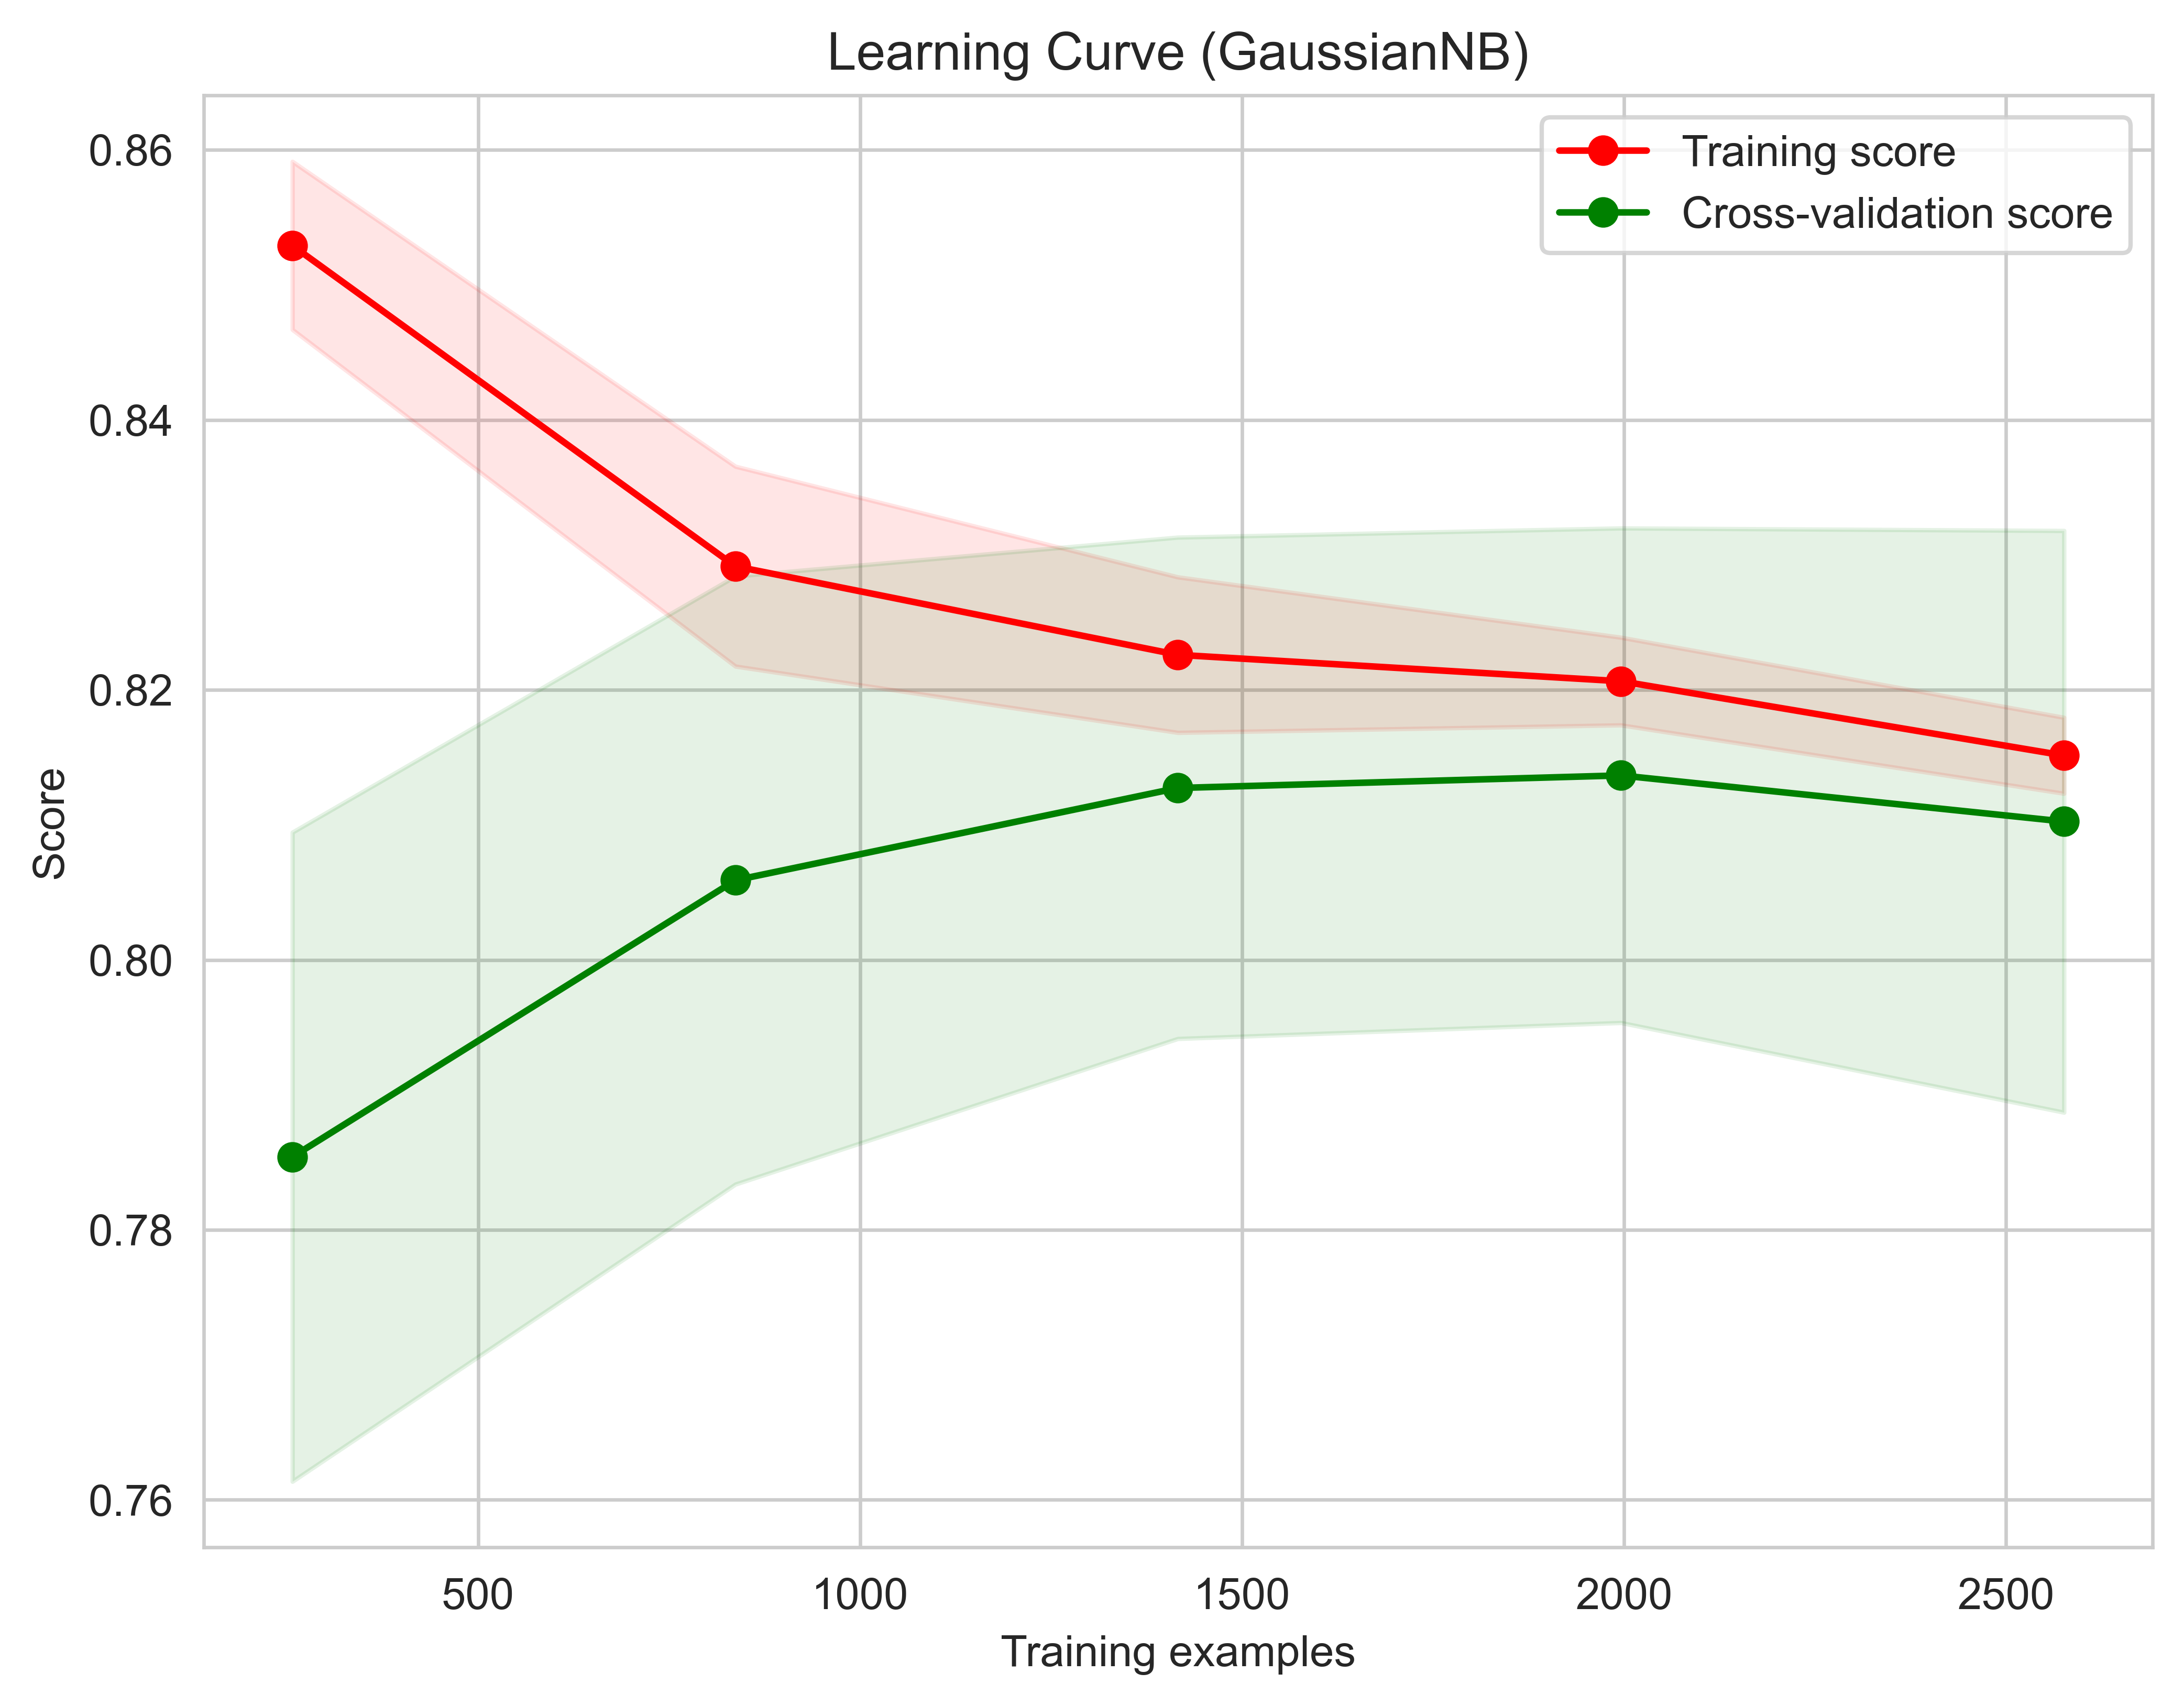
\includegraphics[width=0.8\textwidth]{png/learning_curve_nb.png}
\caption{Learning Curve Analysis - Naive Bayes Classifier}
\end{figure}

\begin{figure}[H]
\centering
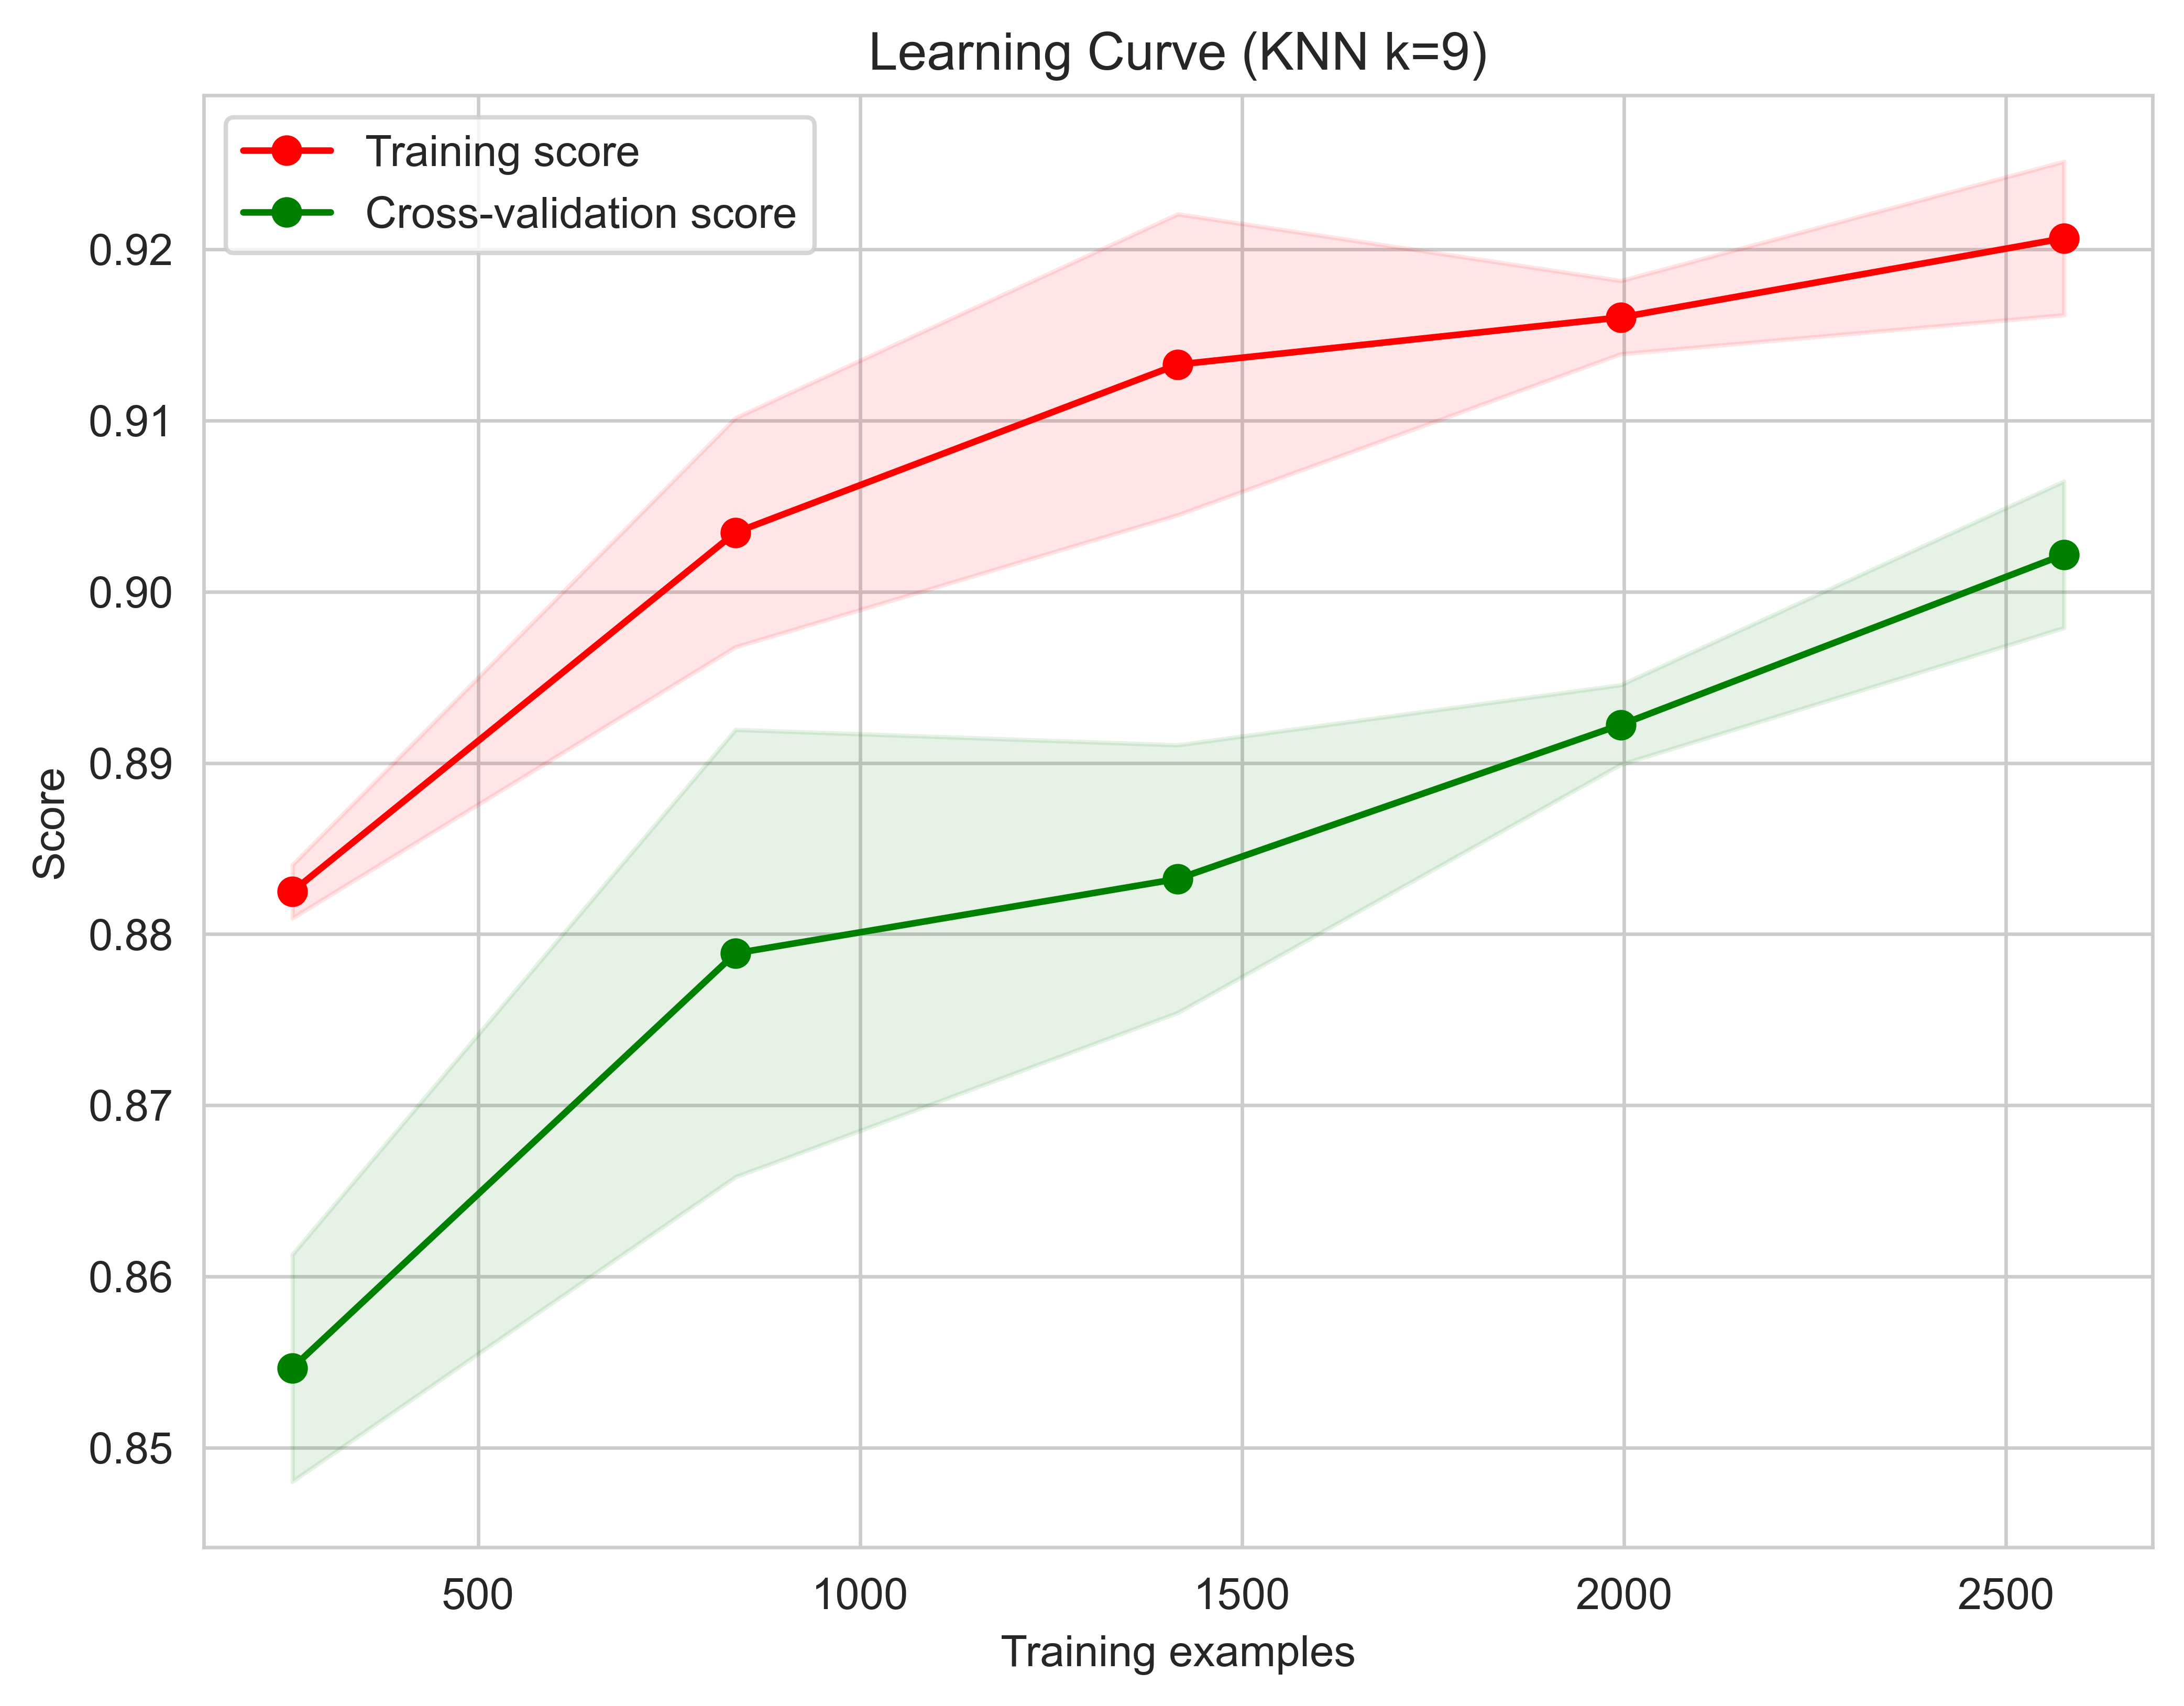
\includegraphics[width=0.8\textwidth]{png/learning_curve_knn.png}
\caption{Learning Curve Analysis - K-Nearest Neighbors}
\end{figure}

%==================================================
\section*{6. Performance Tables}

\subsection*{Na\"ive Bayes Performance Comparison}
\begin{table}[H]
\centering
\renewcommand{\arraystretch}{1.3}
\caption{Comprehensive Performance Metrics for Na\"ive Bayes Variants}
\begin{tabular}{|l|c|c|c|}
\hline
Metric & Gaussian NB & Multinomial NB & Bernoulli NB \\
\hline
Accuracy & 0.8197 & 0.8965 & 0.9030 \\
Precision & 0.7001 & 0.9293 & 0.9100 \\
Recall & 0.9485 & 0.7978 & 0.8364 \\
F1 Score & 0.8056 & 0.8586 & 0.8716 \\
Specificity & 0.7360 & 0.9606 & 0.9462 \\
Training Time (s) & 0.0033 & 0.0016 & 0.0058 \\
\hline
\end{tabular}
\end{table}

\subsection*{KNN Hyperparameter Tuning Results}
\begin{table}[H]
\centering
\renewcommand{\arraystretch}{1.3}
\caption{Optimal Hyperparameters Identified Through Search Methods}
\begin{tabular}{|c|c|c|c|}
\hline
Search Method & Best $k$ & Best CV Accuracy & Best Parameters \\
\hline
Grid Search & 9 & 0.9180 & \{'n\_neighbors': 9, 'weights': 'distance'\} \\
Randomized Search & 9 & 0.9180 & \{'n\_neighbors': 9, 'weights': 'distance'\} \\
\hline
\end{tabular}
\end{table}

\subsection*{KNN Performance using Different Spatial Data Structures}

\begin{table}[H]
\centering
\renewcommand{\arraystretch}{1.3}
\caption{KNN Performance Metrics using KDTree Algorithm}
\begin{tabular}{|l|c|}
\hline
Metric & Value \\
\hline
Optimal $k$ & 9 \\
Accuracy & 0.9180 \\
Precision & 0.9010 \\
Recall & 0.8842 \\
F1 Score & 0.8925 \\
Training Time (s) & 0.0070 \\
Prediction Time (s) & 0.0268 \\
\hline
\end{tabular}
\end{table}

\begin{table}[H]
\centering
\renewcommand{\arraystretch}{1.3}
\caption{KNN Performance Metrics using BallTree Algorithm}
\begin{tabular}{|l|c|}
\hline
Metric & Value \\
\hline
Optimal $k$ & 9 \\
Accuracy & 0.9180 \\
Precision & 0.9010 \\
Recall & 0.8842 \\
F1 Score & 0.8925 \\
Training Time (s) & 0.0054 \\
Prediction Time (s) & 0.0388 \\
\hline
\end{tabular}
\end{table}

\subsection*{Comparative Analysis: KDTree vs BallTree}
\begin{table}[H]
\centering
\renewcommand{\arraystretch}{1.3}
\caption{Efficiency Comparison of Spatial Search Algorithms}
\begin{tabular}{|l|c|c|}
\hline
Criterion & KDTree & BallTree \\
\hline
Accuracy & 0.9180 & 0.9180 \\
Training Time (s) & 0.0070 & 0.0054 \\
Prediction Time (s) & 0.0268 & 0.0388 \\
Memory Usage & Low to Medium & Medium to High \\
Best Use Case & Low-Med Dimensions & High Dimensions \\
\hline
\end{tabular}
\end{table}

%==================================================
\section*{7. Overfitting and Underfitting Analysis}
The learning curve analysis reveals important insights into model generalization capabilities. The KNN classifier with optimal $k=9$ and distance-based weighting demonstrates superior generalization compared to Gaussian Na\"ive Bayes, as evidenced by the convergence of training and validation accuracy curves. The relationship between $k$ and model complexity is inverse: as $k$ increases, the decision boundary becomes smoother and the model exhibits higher bias (potential underfitting), while small $k$ values create complex, irregular boundaries leading to high variance (potential overfitting). The selected optimal value $k=9$ represents a carefully balanced point in the bias-variance tradeoff.

The minimal gap between training and validation scores in the learning curves indicates that the model is not significantly overfitting, suggesting that the regularization effect of $k=9$ is appropriate. For Na\"ive Bayes variants, the Gaussian model shows larger gaps between training and validation performance, indicating its strong independence assumptions may not adequately capture the feature dependencies in the spam detection task. In contrast, Multinomial and Bernoulli variants demonstrate better generalization, likely due to their more appropriate distributional assumptions for frequency-based text features.

%==================================================
\section*{8. Bias--Variance Tradeoff Analysis}
The bias-variance decomposition reveals fundamental differences between parametric and non-parametric approaches. Na\"ive Bayes classifiers, particularly the Gaussian variant, exhibit higher bias due to their strong conditional independence assumptions. These assumptions posit that feature values are independent given the class label, which rarely holds perfectly in real-world text data where word co-occurrences often carry semantic meaning. However, this high bias is accompanied by low variance, meaning Na\"ive Bayes models require relatively small training datasets to achieve stable performance and are less susceptible to overfitting.

K-Nearest Neighbors, as a non-parametric method, demonstrates contrasting characteristics with typically lower bias but higher variance. The absence of strong distributional assumptions allows KNN to model complex decision boundaries, but this flexibility comes at the cost of requiring larger training datasets for the validation performance to converge with training performance. The learning curves confirm this behavior, showing slower convergence for KNN compared to Na\"ive Bayes variants.

Hyperparameter tuning through cross-validated grid search effectively reduces variance in KNN by identifying an appropriate neighborhood size. The distance-based weighting scheme further improves performance by giving more influence to closer neighbors, creating a smoother decision boundary while maintaining flexibility. The convergence of both grid search and randomized search to identical optimal parameters ($k=9$, distance weighting) validates the robustness of the tuning process.

%==================================================
\section*{9. Comprehensive Observations and Conclusion}
This experimental investigation demonstrates several key findings regarding binary classification performance. The K-Nearest Neighbors classifier with $k=9$ achieved the highest classification accuracy of 91.80\%, outperforming all Na\"ive Bayes variants. Among the Na\"ive Bayes family, Bernoulli Na\"ive Bayes (90.30\% accuracy) and Multinomial Na\"ive Bayes (89.65\% accuracy) substantially exceeded Gaussian Na\"ive Bayes (81.97\% accuracy). This performance hierarchy suggests that the word frequency features in the Spambase dataset are more appropriately modeled by discrete probability distributions rather than continuous Gaussian distributions, even after normalization.

The superior performance of Bernoulli and Multinomial variants can be attributed to their alignment with the underlying data generation process. Email spam detection inherently involves analyzing the presence and frequency of specific words and characters, which naturally fit discrete distributional models. The Gaussian assumption of continuous, normally distributed features fails to capture the discrete, count-based nature of word occurrences.

While KNN provided the best predictive accuracy, this performance advantage comes with computational costs. Na\"ive Bayes models demonstrated exceptional computational efficiency, with training times ranging from 1.6ms to 5.8ms and negligible prediction overhead. This efficiency makes Na\"ive Bayes particularly attractive for real-time spam filtering applications where rapid classification of incoming emails is critical. The KNN classifier, despite achieving higher accuracy, requires storing the entire training dataset and computing distances to multiple neighbors for each prediction, resulting in higher memory requirements and inference latency.

The comparison between KDTree and BallTree spatial data structures reveals that KDTree provides faster prediction times (26.8ms vs 38.8ms) for this medium-dimensional dataset (57 features), while BallTree showed slightly faster training (5.4ms vs 7.0ms). This finding aligns with theoretical expectations that KDTree performs efficiently in lower to medium dimensional spaces, whereas BallTree advantages become apparent only in high-dimensional settings or with non-Euclidean distance metrics.

In conclusion, the choice between KNN and Na\"ive Bayes should be guided by the specific application requirements. For scenarios prioritizing maximum accuracy and where computational resources are available, KNN with optimized hyperparameters represents the superior choice. For applications requiring rapid, scalable classification with acceptable accuracy, Bernoulli or Multinomial Na\"ive Bayes provides an excellent balance of performance and efficiency. This experiment successfully demonstrates the importance of algorithm selection, hyperparameter optimization, and understanding the bias-variance tradeoff in developing effective machine learning solutions.

%==================================================
\section*{References}
\begin{itemize}
    \item Scikit-learn Documentation: \href{https://scikit-learn.org/stable/modules/naive_bayes.html}{Na\"ive Bayes Classifiers}
    \item Scikit-learn Documentation: \href{https://scikit-learn.org/stable/modules/neighbors.html}{Nearest Neighbors Algorithms}
    \item Scikit-learn Documentation: \href{https://scikit-learn.org/stable/modules/grid_search.html}{Hyperparameter Optimization Strategies}
    \item UCI Machine Learning Repository: Spambase Dataset
    \item Kaggle: \href{https://www.kaggle.com/datasets/somesh24/spambase}{Spambase Dataset}
    \item Hastie, T., Tibshirani, R., \& Friedman, J. (2009). The Elements of Statistical Learning: Data Mining, Inference, and Prediction. Springer.
    \item Mitchell, T. M. (1997). Machine Learning. McGraw-Hill.
\end{itemize}

\end{document}